\section{Related Works and Motivation}
As analyzed in literature review before this report, traditional schemes for detecting wildfire early and analyzing wildfire actions are based on the features of wildfire smoke and flame. And, deep-neural-network-based (DNN-based) schemes focus more on the feature-learning processes in recent years. In this section, the state-of-art of NN-based wildfire detection and wildfire spreading predictions are studied.
% Fig.~\ref{fig:features} illustrated the commonly used features of smoke and flame for training these DNN models.
% \begin{figure}[ht]
%     \centering
%     \begin{subfigure}{.58\linewidth}
%     \centering
%         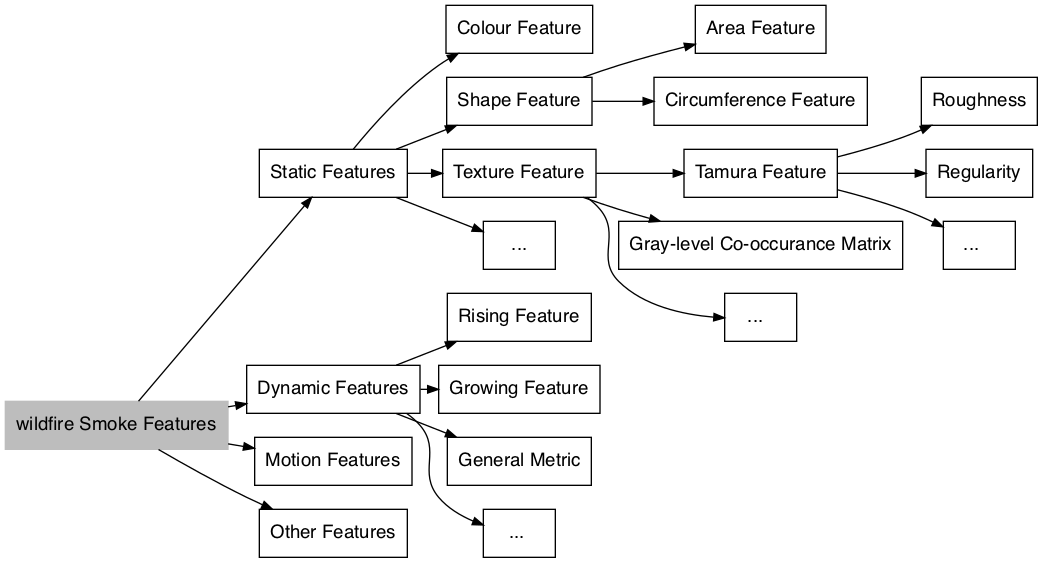
\includegraphics[height = 55mm]{figs/figuresmokefeatures.png}
%         \caption{}
%     \end{subfigure}
%     \begin{subfigure}{.4\linewidth}
%     \centering
%         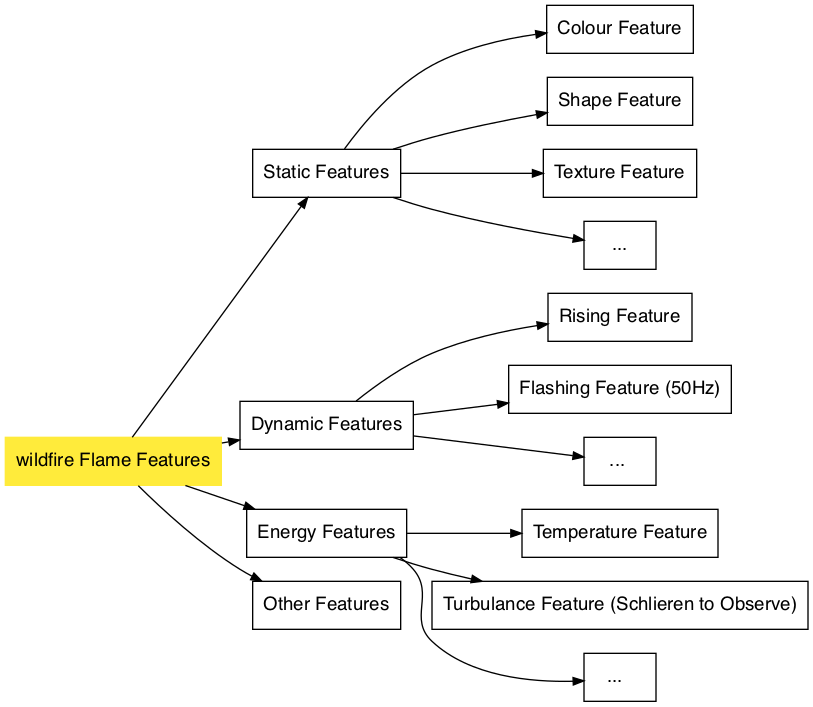
\includegraphics[height = 61mm]{figs/figureflamefeatures.png}
%         \caption{}
%     \end{subfigure}
%     \caption{Commonly applied smoke features and flame features for image-processing-based wildfire detection and analysis. (a) The commonly used smoke features for wildfire detection. (b) The commonly used flame features for wildfire detection.}
%     \label{fig:features}
% \end{figure}
\par
\subsection{NN-based Wildfire Detection Schemes}
For wildfire detection and other recognition tasks, DNNs are higher recommended. Generally, deep networks ensured higher level features could be extracted and better generalized. Also, with the help of transfer learning, it is easier to build segmentation network models for wildfire detection. U-net, one typical fully connected network (FCN) is widely accepted and applied in wildfire detection \cite{li2019detection, park2020wildfire, he2016deep, huang2017densely, mommert2020characterization}. There are also region-based convolutional network (R-CNN) \cite{lee2019deep} and recurrent neural network (RNN) \cite{jeong2020light} models could finish sequence-to-sequence analysis of wildfire data to detect smoke or flame.\par
However, in the most recent research, it is found that layers in these models are more computational complex. Because of the demand of early detection. The networks are often considered to be deployed on-board for UAV or UAVs. Saving the computing resource and simplifying the structure of networks are very challenging.\par 
Under such situation, light network models are studied. In \cite{peng2019real}, depthwise seperable convolution and SqueezeNet are considered to build blocks called fire model to detect wildfire. Based on fire models, a light U-net is proposed \cite{zhang2021att} to share parameters and save computing resources. on the other hand, attention mechanism is demonstrated that they could keep more deeper information in the down sampling process and decreased false positive detection \cite{oktay2018attention}. Also, it is found that attention layers is lower computational complexity by comparing with convolutional layer \cite{vaswani2017attention} in the research of Transformer. Vision transformer (ViT) model demonstrated that attention mechanism performed well in higher-resolution tasks \cite{zhang2018image}.\par
However, the application of attention mechanism also has its challenges. For example, for sequence data set, attention could not capture the order information, which limited the attention to learn partial information. These researches motivated the design and implementation to optimize the encoder-decoder structured model or models combining with attention mechanism for wildfire detection to save more computational resource and perform more meticulous and accurate segmentation.
\subsection{Wildfire Prediction Schemes}
After detecting the wildfire, it is also important to understand the dynamics and actions of wildfire, which motivated the study of wildfire spreading models. For a long period, wildfire spreading prediction are mainly rely on two typical numerical model:\par
The fist one is based on physical modeling accounting for various physical and chemical phenomena. This kind of model contains computational-fluid-dynamics (CFD) \cite{mueller2014large} which could describe the spreading progress with more details. However, its performance on real fire still need more discussion because of high computational cost and the environmental complexity.\par
The second one is the mathematical model which based on empirical model of rate of spread (RoS). As illustrated in \cite{alexandridis2008cellular}, mathematical growth prediction models is an acceptable description for wildfire spreading. Similar as fire area simulator (FARSITE) \cite{finney1999farsite}, a type consists of models based on continuous plane assumed the fire spreads in a continuous landscape and solving a system of partial differential equations is considered as the solution of these models\cite{richards1995general}. A computationally faster type consists of the models based on grid \cite{pastor2003mathematical}. Typically, there are Cellular Automata (CA) \cite{trunfio2004predicting} and Bond-Percolation method. Compared with Bond-percolation method, CA solved its problem of describing the dynamics of the fire spread. There are also some other types of models, such as the fuzzy or neural based ones \cite{vakalis2004gis1,vakalis2004gis2}.\par
\begin{figure}[ht]
    \centering
    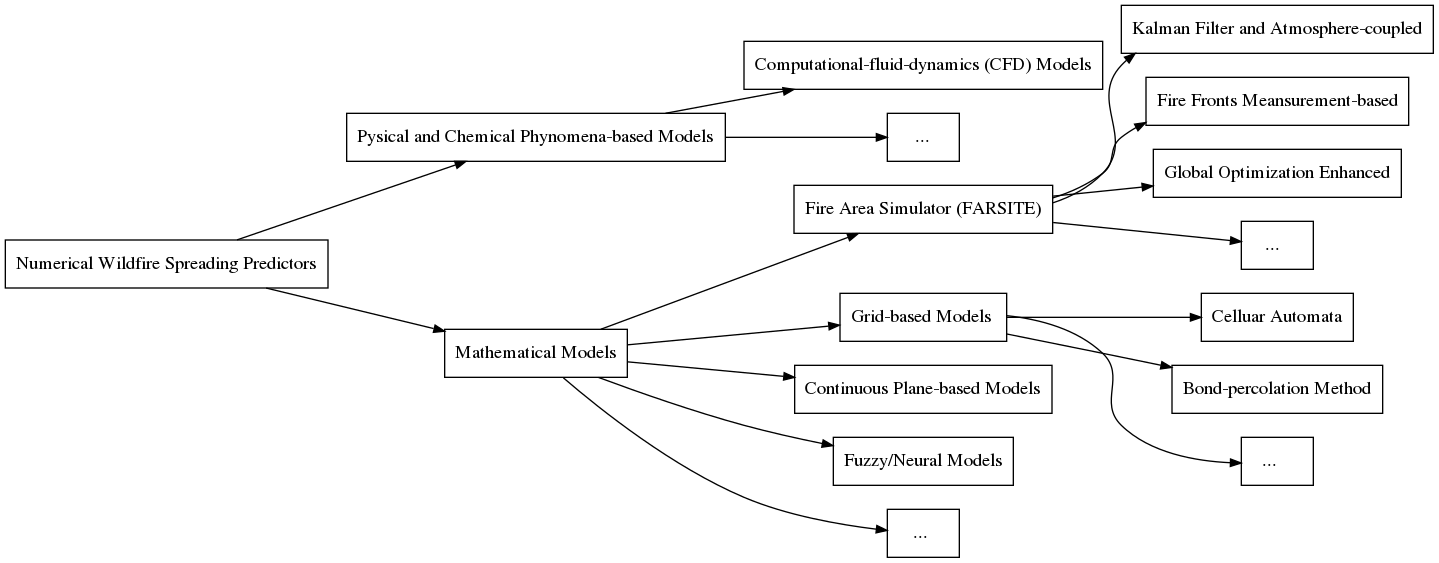
\includegraphics[height=68mm]{figs/figurepredictionmodel.png}
    \caption{Main schemes for predicting the wildfire spread}
    \label{fig:spreadmodel}
\end{figure}
Generally, data-driven schemes could be applied for improving the accuracy of locating fire fronts and reduce the simulation uncertainty. In the review \cite{zhai2020learning}, Kalman filter, Lagrangian particle, Huygens principle and level-set method are mentioned to predict the fire front based on the real-time RoS measurement.
The aforementioned schemes could be illustrated in Fig.~\ref{fig:spreadmodel}. In recent years, it is found that data collected from geographic information system (GIS) and data augmentation with some NN models are also helpful in building these models. For example, the performance of FireCast of 2D-CNN \cite{radke2019firecast} and LSTM \cite{huot2020deep} both encouraging.\par 
However, these models often work for a relatively large time step (hours or days) \cite{burge2020convolutional}. The complex forest environment might change rapidly during the early fire period. To improve the accuracy and prediction speed need more investigation and demonstration. Such objectives motivated that the application of probabilistic models \cite{pimont2021prediction}, attention mechanism \cite{vaswani2021scaling}, and some popular DNN models to be applied.\par
\subsection{Vision-based Wildfire Tracking Schemes}
The prediction schemes mentioned above could be treated as a kind of auto-regressive processes. However, they are nearly to predict the wildfire scar, where the vegetation are already burnt, improving the accuracy of the fire front prediction is much more challenging for such indirect schemes by considering the wind-slope and other interacting factors. The accuracy and sensitiveness limitations are considered. Therefore, remote-sensing (equipped UAV) supported fire fronts tracking is thought about to ensure the predictions and monitoring of suspected wildfire areas.\par
Commonly, in forest fire management, visual object tracking (VOT) is the most efficient tracking scheme, VOT is studied in this research. VOT could be evaluated through OTB50 or OTB100 benchmarks \cite{wu2013online}. The mainly applied VOT scheme consists of traditional 
% 迭代模型
generative model (GM),
% 判别模型
discriminative model (DM),
% deep learning model
and the DNN-based model getting hot in recent years. 
Commonly, GM build the objective model or extract the objective features at first, then it would search the similar features in the coming frames, and iterated to locate the tracking target. However, the background information and the randomness and multiple shape changing of target are not efficiently used when it is used in environment where it is lower resolution, brightness changing, which limited its accuracy in wildfire management. Compared with GM, DM performs better in mean frame per second (FPS) and mean precision. DM extracts and locates the target in local frame by comparing the different information of target and background. Related filters and some machine learning based classifiers are being applied as DM for VOT. Also, there is DNN-based model, which is different from GM and DM \cite{krebs2017survey}. These main schemes could be illustrated in Fig.~\ref{fig:figuretrackingmodel}.
\begin{figure}[ht]
    \centering
    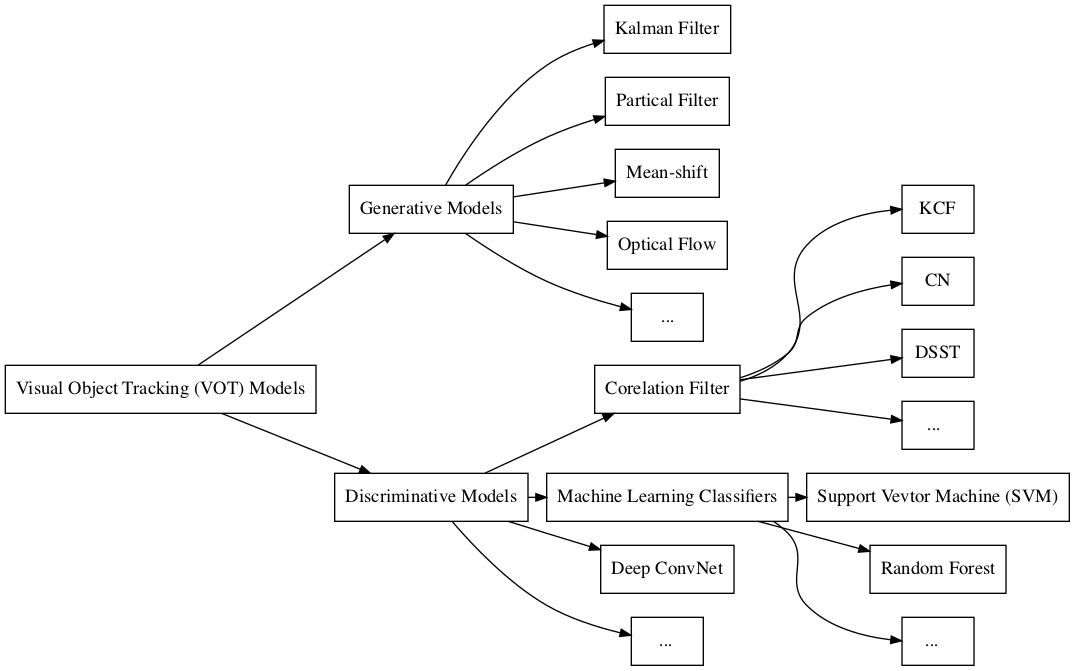
\includegraphics[height=80mm]{figs/figuretrackingmodel.png}
    \caption{Main schemes could be applied for tracking fire fronts}
    \label{fig:figuretrackingmodel}
\end{figure}
\par
With the support of VOT, UAV or UAVs could track or avoid the smoke and flame area and give fire fighters more information in wildfire management tasks. The 
\vspace{-0.3cm}
